\documentclass{article}

% if you need to pass options to natbib, use, e.g.:
%     \PassOptionsToPackage{numbers, compress}{natbib}
% before loading neurips_2024


% ready for submission
\usepackage{neurips_2024}
\usepackage{natbib}

\usepackage{graphicx}
\usepackage[utf8]{inputenc} % allow utf-8 input
\usepackage[T1]{fontenc}    % use 8-bit T1 fonts
\usepackage{hyperref}       % hyperlinks
\usepackage{url}            % simple URL typesetting
\usepackage{booktabs}       % professional-quality tables
\usepackage{amsfonts}       % blackboard math symbols
\usepackage{nicefrac}       % compact symbols for 1/2, etc.
\usepackage{microtype}      % microtypography
\usepackage{xcolor}         % colors


\title{Escherichia Coli Ceftriaxone Resistance}

% The \author macro works with any number of authors. There are two commands
% used to separate the names and addresses of multiple authors: \And and \AND.
%
% Using \And between authors leaves it to LaTeX to determine where to break the
% lines. Using \AND forces a line break at that point. So, if LaTeX puts 3 of 4
% authors names on the first line, and the last on the second line, try using
% \AND instead of \And before the third author name.

\author{%
  D. Bugatti, N. Dupertuis, A. Giacomuzzi, N. Oberholzer\\
  Foundations of Data Science\\
  Department of Health Science and Technology\\
  ETH Zürich\\
}



\begin{document}
\maketitle

\begin{abstract}
Antibiotic resistance is a growing global health threat, requiring fast and accurate diagnostic tools to guide treatment decisions. In this project, we examine the resistance of Escherichia coli to Ceftriaxone using MALDI-TOF mass spectrometry data from the DRIAMS dataset. The dataset contains 1368 clinical samples with 5999 spectral features. We apply and compare four machine learning models: Support Vector Machine (SVM), Logistic Regression, Random Forest, and k-Nearest Neighbors (kNN). Feature selection and class imbalance handling are used to improve predictive performance. Logistic Regression achieved the highest overall accuracy and ROC AUC, while Random Forest showed perfect recall, illustrating trade-offs between sensitivity and specificity. These results highlight the potential of MALDI-TOF spectral data for predicting antibiotic resistance in E. coli and demonstrate how machine learning can support rapid diagnostics. The study also points to key deployment considerations, such as model robustness and interpretability, that are critical for real-world clinical applications.
\end{abstract}


\section{Introduction}

Antibiotic resistance is a rapidly escalating global health threat, significantly complicating the treatment of bacterial infections and leading to higher mortality, morbidity, and healthcare costs worldwide. Recent data underscore the severity of this issue; for example, a systematic review conducted by \citet{IranBacteria} revealed that 87.5\% of bacterial isolates obtained from clinical specimens in Northern Iran showed resistance to at least one commonly prescribed antibiotic. Given ongoing selective pressure, this alarming prevalence is likely even higher today, emphasizing the critical need for effective diagnostic tools to rapidly identify resistant strains and guide therapeutic decisions.

Matrix-Assisted Laser Desorption/Ionization Time-of-Flight (MALDI-TOF) mass spectrometry has emerged as a powerful technique for rapid microbial identification and characterization. A recent large-scale study compiled MALDI-TOF mass spectra from over 300,000 bacterial and fungal samples and successfully applied machine learning techniques to predict antimicrobial resistance phenotypes directly from these spectra \citep{datasetExplaination}. Leveraging such techniques could significantly reduce the time required for identifying resistance profiles compared to traditional phenotypic testing methods.

In this project, we specifically focus on evaluating the predictive capabilities of classical machine learning models—Support Vector Machine (SVM), Logistic Regression, Random Forest, and k-Nearest Neighbors (kNN)—for detecting Ceftriaxone resistance in \textit{Escherichia coli} using MALDI-TOF spectra from the publicly available DRIAMS dataset. Our primary aim is to assess the real-world applicability and performance of these machine learning algorithms in accurately distinguishing Ceftriaxone-resistant strains from sensitive ones.

The scientific hypothesis tested in this study is that classical machine learning algorithms, trained on MALDI-TOF spectral data, can achieve clinically relevant performance (ROC AUC > 0.85) in predicting Ceftriaxone resistance in \textit{Escherichia coli}.

\section{Methods}

\subsection{Data Wrangling and Visualization}
\textbf{\textit{Maybe add Data source? 
}}The dataset consists of an integer label, either 1 or 0, indicating resistance to the antibiotic; mass
spectrometry results, which are floats ranging from 0 to 1, which have been most likely normalized; and a
column named ”Unnamed : 0” which has elements of type string. This column contained a serial number
ending with either “MALDI\_1” or “MALDI\_2”, suggesting it might relate to the machines used for the
observations. To prevent overfitting, we decided to remove this column. Additionally, we checked the
dataset for NA and duplicates but found none. The reformatted dataset now consists in 5999 features
and one label spanning over 1386 samples. 

\subsubsection{Avoiding the Curse of Dimensionality}

As the dataset contains more features than samples, a feature
selection must be performed before fitting with either a filter, wrapper or embedded method. To ensure
that some features can be removed without losing too much information, we created a Pearson’s correlation
matrix of the features and plotted its heatmap with matplotlib \citep{matplotlib} and seaborn \citep{seaborn}.\\

\begin{figure}
	\centering
	\includegraphics[width=0.9\textwidth]{heatmap.png}
	 \vspace{-3em}
	\caption{Heatmap of Pearson's correlation matrix}
\end{figure}

Except the trivial white line that divides the heatmap in half, there are numerous white and dark blue spots, which indicate high positive or negative correlation. Thanks to the graph we can safely assume that most of the variable are correlated, and therefore a filter will not only diminish the probability of overfitting (as mentioned earlier, a higher number of features than samples must always be avoided), but also focus the attention of the model onto non-collinear and highly explanatory features. 

\subsubsection{Assessing Class Imbalance}

Another issue that must be addressed is the class imbalance; 81.5\% of the bacteria samples are resistant to Ceftriaxone, and only 18.5\% are not. There are several ways to help the model focus more onto the minority class. One solution is undersampling the majority class, but we ruled this out, because our dataset already has a relatively low number of samples. Another solution is oversampling the minority, but we rejected it because the duplicated samples would have identical values, therefore increasing the chance of overfitting which is already a concern with this dataset. The solution we chose as best is balancing the class weight in the model. This method doesn't involve dataset alterations, it instead adjusts the training process by giving more importance to mistakes made on the minority class. Specifically, by multiplying such errors by a weight, usually set inversely proportional to the minority class frequency.

\subsubsection{Dataset Split}

The dataset has been split into training and testing sets with an 85\% ratio for training and a 15\% ratio for testing. This leaves 208 samples for testing and 1178 samples for training.

\subsection{Models}
\subsubsection{SVM}
Text here

\subsubsection{Random Forest}
Random Forest (RF) is an ensemble learning algorithm that builds multiple decision trees during training and outputs the class that is the mode of the classes predicted by individual trees. Random Forest was selected for its robustness to noisy and high-dimensional datasets, ease of use, and inherent handling of non-linear relationships without extensive data preprocessing.

To optimize model performance, we performed hyperparameter tuning using grid search with 5-fold cross-validation. The hyperparameters considered were:

\begin{itemize}
    \item \textbf{Number of Trees (\texttt{n\_estimators})}: [300, 350, 400, 450, 500].
    \item \textbf{Maximum Tree Depth (\texttt{max\_depth})}: [None, 10, 20].
    \item \textbf{Minimum Samples for Node Splitting (\texttt{min\_samples\_split})}: [2, 5, 10].
\end{itemize}

To address the significant class imbalance present in the dataset (81.5\% resistant vs. 18.5\% sensitive), the parameter \texttt{class\_weight="balanced"} was set, ensuring increased penalization of misclassification errors for the minority class during training.

Hyperparameter tuning was evaluated using the Receiver Operating Characteristic Area Under the Curve (ROC AUC), specifically selected for its effectiveness in evaluating models trained on imbalanced datasets. This aligns with our aim of achieving clinically relevant predictive performance (ROC AUC > 0.85).

\subsubsection{Logistic Regression}
Text here

\subsubsection{K Nearest Neighbors}
Text here


\subsection{Evaluation Metrics}

Given the highly imbalanced nature of our dataset (81.5\% resistant vs. 18.5\% sensitive samples), standard accuracy alone is insufficient to reliably evaluate predictive performance. To address this, we employed multiple complementary evaluation metrics specifically chosen for their effectiveness in assessing performance on imbalanced data:

\begin{itemize}
    \item \textbf{ROC AUC (Receiver Operating Characteristic Area Under the Curve):} 
    ROC AUC provides a robust measure of model performance independent of the classification threshold, specifically capturing the model's ability to distinguish between resistant and sensitive cases. A ROC AUC greater than 0.85 was predefined as clinically relevant.

    \item \textbf{Precision:} Precision is the proportion of positive identifications (predicted resistant) that are actually resistant. High precision ensures that the model minimizes false positives, reducing unnecessary or inappropriate treatments.

    \item \textbf{Recall (Sensitivity):} Recall is the proportion of actual resistant cases correctly identified by the model. High recall is crucial clinically, as failing to identify a resistant strain can lead to ineffective treatment.

    \item \textbf{F1 Score:} The harmonic mean of precision and recall provides a balanced measure of performance when classes are imbalanced, reflecting the trade-off between precision and recall clearly.

    \item \textbf{Accuracy:} While accuracy provides an overall performance summary, it should be interpreted cautiously due to its bias in imbalanced scenarios. We include it primarily as a baseline reference.
\end{itemize}

These metrics collectively provide a comprehensive evaluation of each model, enabling clear insight into the practical strengths and weaknesses of each approach.

\section{Results}

The following models have been trained and evaluated on the same dataset split, enabling an equal comparison and evaluation of their performance. They have been developed with Scikit-learn's \citep{scikit-learn}, Pandas's \citep{pandas} and numpy's \citep{numpy} algorithms and documentations. 

\subsection{SVM}

Support Vector Machine (SVM) makes his prediction based on hyperplane divisions on the multidimensional feature space. It is therefore extremely important for the success of the model, to select only the highly explanatory features. 

\subsubsection{Model Workflow Explanation}

We created a flowchart which should help visualize the model.

\begin{figure}[h]
	\centering
	\includegraphics[width=1.0\textwidth]{FlowChart.png}
	 \vspace{0em}
	\caption{Flowchart of the implemented SVM Model}
\end{figure}

As SVM is so dependent on the selected features, we decided to implement a wrapper method which unifies feature selection and SVM model tuning into a grid search cross validation environment to iterate the method for every combination of hyperparameters possible for both feature selection and SVM. At first, a number K of features are selected to train the SVM. The non selected features are discarded. The selection algorithm we deemed best is ANOVA, because it selects the features whose variance contributes the most to the variance in the label. Since SVMs require highly explanatory features, this selection method aligns perfectly with their requirements. After the filtering process, a Support Vector Machine (SVM) model is fitted with a combination of two hyperparameters: C, which represents the strength of the penalty applied through L2 regularization, and Kernel, which determines the shape of the division between classes.

Thanks to pipelining, the same grid search cross validation (5 folds) was used to iterate between all of the combinations of the three hyperparameters:
 
\begin{itemize}
  \item Feature selection's K: [500, 1000, 1250, 1500, 1750]
  \item SVM's C: [10, 100, 125, 150, 175]
  \item SVM's Kernel: ["linear", "poly", "rbf", "sigmoid"]
\end{itemize}

The best model was then selected using the average from each fold of the ROC AUC score. 

\subsubsection{Model Evaluation}

The model that performed the best during cross validation was an SVM with rbf kernel and C coefficient equal to 125 fitted on 1500 out of the 5999 total features. After retraining the model on the whole training dataset, we evaluated on the test dataset and obtained the following results:

\begin{figure}[h]
	\centering
	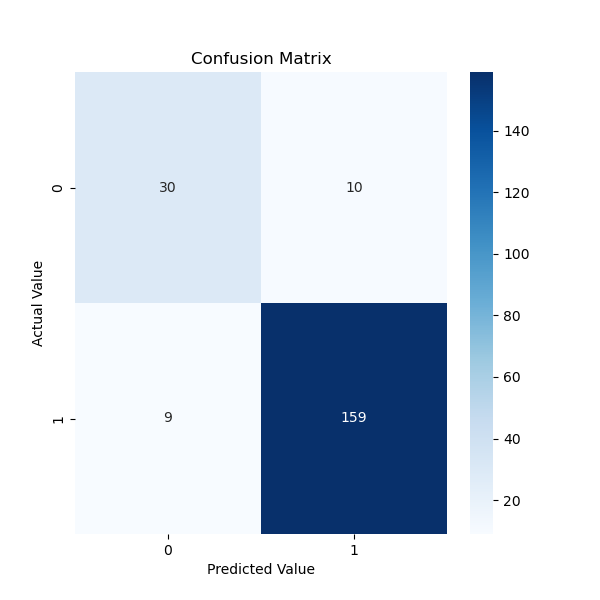
\includegraphics[width=0.6\textwidth]{confusion_matrix_SVM.png}
	 \vspace{-1em}
	\caption{Confusion Matrix of the SVM}
\end{figure}

The statistics calculated from the confusion matrix are the following: 
\begin{itemize}
  \item Accuracy:   0.9086538461538461
  \item Precision:   0.9408284023668639
  \item Recall:   0.9464285714285714
  \item F1:   0.9436201780415431
\end{itemize}
Accuracy is the lowest of the scores, and this is explained by looking at the confusion matrix. The model is quite good at predicting positive bacteria samples, but performs quite worse in predicting negative samples. As accuracy gives the same importance to both positive and negative samples, it is comprehensibly the lowest score. The calculated ROC AUC score was instead a 0.9149. Overall, the model performed reasonably well, however there still might be space for improvements on the hyperparameters.
Since the filtering process was itself part of the model and caused the model to perform better, it is not only fair, but also right to compare the model with specific feature selection with the other models, which have selected their features in a different way.

\subsection{Random Forest}

The optimal hyperparameter combination found through cross-validation was:
\begin{itemize}
    \item \texttt{n\_estimators} = 500
    \item \texttt{max\_depth} = 20
    \item \texttt{min\_samples\_split} = 5
\end{itemize}

The optimized Random Forest model was retrained on the entire training set (1178 samples) and evaluated on the test set (208 samples). Figure \ref{fig:rf_confusion_matrix} illustrates the confusion matrix for the Random Forest classifier on the test dataset.

\begin{figure}[h]
  \centering
  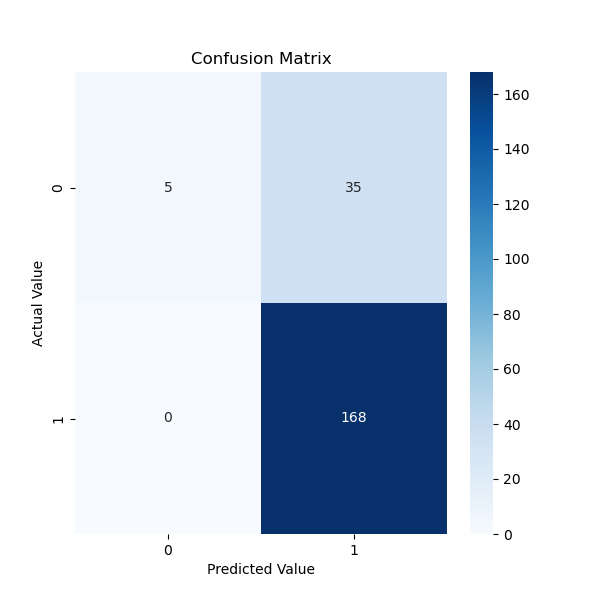
\includegraphics[width=0.6\textwidth]{confusion_matrix_Random_Forest.png}
  \caption{Confusion Matrix for the Random Forest classifier on the test dataset. Class labels: 0 = Sensitive, 1 = Resistant.}
  \label{fig:rf_confusion_matrix}
\end{figure}

From the confusion matrix, the following performance metrics were calculated:

\begin{table}[h]
\centering
\caption{Random Forest Performance Metrics}
\begin{tabular}{lr}
\toprule
\textbf{Metric} & \textbf{Score} \\
\midrule
ROC AUC   & 0.8192 \\
Accuracy  & 0.8317 \\
Precision & 0.8267 \\
Recall    & 1.0000 \\
F1 Score  & 0.9051 \\
\bottomrule
\end{tabular}
\end{table}

The Random Forest model demonstrated a perfect recall (1.0), correctly identifying all resistant samples. However, this high recall came at the cost of a lower precision (0.8267), indicating a relatively higher false-positive rate. Such a trade-off is crucial to consider in clinical diagnostics, where failing to identify resistant cases could have severe implications.

We also extracted feature importances from the trained model. The most important features were those corresponding to spectral bins 109, 51, 78, and 740, among others. These may relate to biologically meaningful patterns, although further biochemical interpretation would be required.

Overall, Random Forest demonstrated strong generalization performance and robustness to feature selection, with particularly valuable recall in the context of resistance prediction.

\subsection{Logistic Regression}

\subsection{K Nearest Neighbors}

\section{Discussion}

ONLY A DRAFT

Our analysis investigated the use of machine learning models to predict resistance to Ceftriaxone in \textit{Escherichia coli} using MALDI-TOF mass spectrometry data from the DRIAMS dataset. The motivation stems from the pressing global issue of antimicrobial resistance (AMR), which is predicted to cause up to 10 million deaths annually by 2050 if unaddressed \citep{doi:10.1016/S1473-3099(15)70136-9}. Rapid diagnostics, particularly those leveraging high-throughput phenotypic data such as MALDI-TOF, offer promising avenues to inform clinical treatment decisions.

Our dataset consisted of 1368 samples and 5999 spectral features, with a highly imbalanced distribution where ~81.5\% of samples were resistant to Ceftriaxone. We implemented four models—Support Vector Machine (SVM), Random Forest (RF), Logistic Regression (LR), and k-Nearest Neighbors (kNN)—and applied different strategies for feature selection and hyperparameter optimization. The models were evaluated on a held-out test set using metrics such as accuracy, precision, recall, F1 score, and ROC AUC.

The Logistic Regression model, regularized via L1 penalty and paired with forward feature selection, performed best overall in terms of ROC AUC (0.911) and F1 score (0.939). This aligns with findings in the literature such as Weis et al. (2022) \citep{doi:10.1038/s41591-021-01619-9}, where logistic models were also found to perform competitively for AMR prediction when features were appropriately selected. SVM also showed balanced performance (AUC: 0.876), while Random Forest stood out for achieving perfect recall (1.000), correctly identifying all resistant samples. However, its lower precision (0.827) indicated a higher false positive rate, which could reduce clinical efficiency if used in isolation.

In contrast, kNN achieved a high recall (0.958) and F1 score (0.907), but underperformed on ROC AUC (0.797), highlighting the model’s sensitivity to feature scaling and dimensionality. These findings reinforce the need to match model complexity to data characteristics and use case objectives: for example, models prioritizing recall are suitable for initial triage, whereas those maximizing precision may be better for guiding treatment.

\subsection*{Relation to Previous Work}
Our findings build upon the growing body of research leveraging MALDI-TOF spectra for AMR classification. Weis et al. (2022) demonstrated the effectiveness of convolutional neural networks on the same DRIAMS data, reporting AUC values between 0.85 and 0.93 depending on the species-antibiotic pair \citep{doi:10.1038/s41591-021-01619-9}. Our classical models, particularly Logistic Regression and SVM, achieved comparable performance with significantly lower computational overhead and greater interpretability.

Other work, such as Brackmann et al. (2023) \citep{doi:10.1093/cid/ciad080}, emphasizes the practical value of integrating such models into laboratory workflows, particularly in resource-constrained environments where rapid deep learning deployment is less feasible. Our results support these observations and demonstrate that simpler models—when tuned effectively—can be viable alternatives.

\subsection*{Limitations}
There are several limitations to our work:
\begin{itemize}
    \item \textbf{Data Imbalance:} While we applied class weighting, more advanced techniques such as SMOTE or generative augmentation could improve model robustness.
    \item \textbf{Biological Interpretation:} The spectral features used are not annotated with biological markers, limiting interpretability of the most predictive features.
    \item \textbf{Cross-Institution Generalizability:} Our train-test split was random and not stratified by source institution, so real-world generalization to new hospitals is untested.
    \item \textbf{Model Scope:} We only tested four models. Other techniques, such as gradient boosting or neural networks, may provide better results.
\end{itemize}

\subsection*{Outlook}
To further validate the applicability of these models, future work should explore:
\begin{itemize}
    \item \textbf{Cross-institution validation:} Training on data from one hospital and testing on another to test generalizability.
    \item \textbf{Feature interpretation:} Using methods such as SHAP or LIME to link predictive peaks to known resistance genes or protein signatures.
    \item \textbf{Expanded model comparison:} Including deep learning architectures and ensemble methods.
    \item \textbf{Clinical integration:} Assessing model performance when embedded into real diagnostic pipelines.
\end{itemize}

In summary, we demonstrate that classical machine learning models can predict Ceftriaxone resistance in \textit{E. coli} using MALDI-TOF spectra with reasonable performance. Logistic Regression and SVM models offer a good balance between accuracy and interpretability, while Random Forest provides high sensitivity. These results affirm the feasibility of data-driven tools in antimicrobial resistance diagnostics and set a foundation for further study and clinical translation.


\bibliographystyle{plainnat}

\bibliography{bibliography}


\end{document}




%%				cd  /Users/user/Desktop/project/project/report 			pdflatex -shell-escape Report.tex

%%															bibtex report   



























